\documentclass[tikz,convert={outext=.svg,command=\unexpanded{pdf2svg \infile\space\outfile}},multi=false]{standalone}
\usepackage[utf8]{inputenc}


\begin{document}


\newcommand{\cerealbox}{
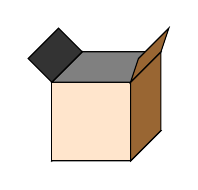
\begin{tikzpicture}[fill=orange,fill opacity=1,draw,scale=1]
	\def\cubecol{blue}
	\def\opacity{0.8}
	\filldraw (-0.5,-0.5,-0.5) -- ++(1,0,0) -- ++(0,1,0) -- ++(-1, 0, 0) -- cycle;
	\filldraw (-0.5,-0.5,-0.5) -- ++(1,0,0) -- ++(0,0,1) -- ++(-1, 0, 0) -- cycle;
	\filldraw (-0.5,-0.5,-0.5) -- ++(0,1,0) -- ++(0,0,1) -- ++(0, -1, 0) -- cycle;
	\filldraw[fill=orange!20] (0.5,0.5,0.5) -- ++(-1,0,0) -- ++(0,-1,0) -- ++(1, 0, 0) -- cycle;
	\filldraw[fill=black!50!black!50] (0.5,0.5,0.5) -- ++(-1,0,0) -- ++(0,0,-1) -- ++(1, 0, 0) -- cycle;
	\filldraw[fill=orange!50!black!80] (0.5,0.5,0.5) -- ++(0,-1,0) -- ++(0,0,-1) -- ++(0, 1, 0) -- cycle;
	\filldraw[fill=orange!50!black!80] (0.5,0.5,0.5) -- ++(0.1,0.3,0) -- ++(0,0,-1) -- ++(-0.1, -0.3, 0) -- cycle;
		\filldraw[fill=black!20!black!80] (-0.5,0.5,0.5) -- ++(-0.3,0.3,0) -- ++(0,0,-1) -- ++(0.3, -0.3, 0) -- cycle;
\end{tikzpicture}}


\def\colorPallete{{"1.0 1.0 1.0", "0.7 0.7 1", "1.0 0.7 0", "1.00 0.98 0.00", "0.1 0.8 0.00"}}



\newcommand{\coupon}[1]{
	\begin{tikzpicture}
		\pgfmathparse{\colorPallete[#1]};
		\definecolor{currentColor}{rgb}{\pgfmathresult};
		\node[draw, rotate=20, inner sep=2mm, minimum height=6mm, fill=currentColor] {\textbf{#1}};
\end{tikzpicture}}

\tikzstyle{col} = [draw]


\newcommand{\collection}[4]{
	\begin{tikzpicture}
		\pgfmathparse{\colorPallete[#1]};
	\definecolor{currentColor}{rgb}{\pgfmathresult};
		\node[col,fill=currentColor] {1};
			\pgfmathparse{\colorPallete[#2]};
		\definecolor{currentColor}{rgb}{\pgfmathresult};
		\node[col, fill=currentColor] at (0, -0.5) {2};
			\pgfmathparse{\colorPallete[#3]};
		\definecolor{currentColor}{rgb}{\pgfmathresult};
		\node[col,fill=currentColor] at (0, -1) {3};
			\pgfmathparse{\colorPallete[#4]};
		\definecolor{currentColor}{rgb}{\pgfmathresult};
		\node[col,fill=currentColor] at (0, -1.5) {4};
	\end{tikzpicture}
}

\newcommand{\boxwith}[5]{
\begin{tikzpicture}
	\node[inner sep=-5mm] (b) {\cerealbox};
	\node[inner sep=0mm] (v) at (1, 2) {\coupon{#1}};
	\draw[-latex] (b) edge[line width=0.6mm, bend left=20] (v);
	\node at (1.8, 1.8) {\collection #2 #3 #4 #5};
	\node at (2.6, -0.8) {};
\end{tikzpicture}
}



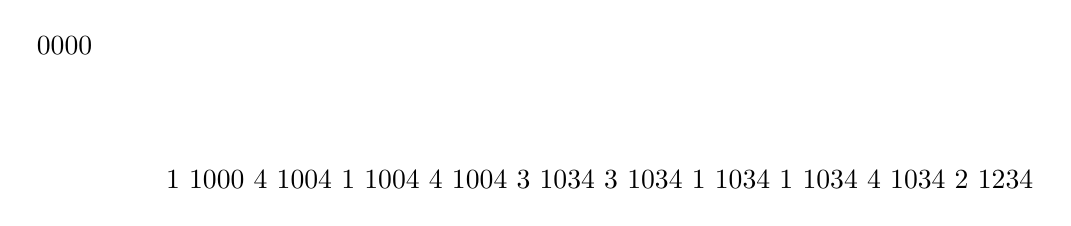
\begin{tikzpicture}
	\node {
		\raisebox{17mm}{\collection 0000} ~~~~~~
		\boxwith1 1000
		\boxwith4 1004
		\boxwith1 1004
		\boxwith4 1004
		\boxwith3 1034
		\boxwith3 1034
		\boxwith1 1034
		\boxwith1 1034
		\boxwith4 1034
		\boxwith2 1234
	};
\end{tikzpicture}

\end{document}